\documentclass{article}
\usepackage{malmacros}
\begin{document}

\section{Keras Multi-Layer Perceptrons on Moon-data}
In this chapter we are working with the Multi-layer perceptrons and we see how using neural networks can speed up and enhance the training of models. We also experiment with how different optimizers can improve the precision of the models trained.

\subsection{Qa Using a Keras MLP on the Moon-data}
In this section a comparison between the currently favored optimizer: \textbf{Adam} (\textit{adaptive moment estimation}) and a good old Stochastic Gradient Optimizer. At first the results are quite far from each other with \textbf{Adam} reaching a score of 96.4 percent. And the \textbf{SGD} optimizer reaching only 88 percent. But in the book around chapter 11 (page. 294) we learn about \textbf{Momentum} optimizers, which changes the Gradient descent steps, from being steps and more like the behaviour of a rolling bowling ball, where it starts slowing and then "picks up" momentum, as it goes. With this it will reach the global minimum faster than standard gradient descent, and the added momentum will help it "roll out" of local minimums, that gradient descent might get stuck in. 
\\ \\
In short the way \textbf{Momentum Optimization} works is opposite to standard Gradient Descent which does not take previous gradients into account, the Momentum does. At each iteration it takes the local gradient and adds it to the \textit{momentum vector} \textbf{m} which is then multiplied by the learning rate and then the weights of the gradient descent are updated by simply subtracting the momentum vector. This then creates this sort of "acceleration".
\\ \\
But why stop here. To further improve the performance and precision of the model. Instead of just using the vanilla Momentum Optimizer, the \textit{Nesterov Momentum Optimization} can be used to increase the speed and precision score. It is also known as the \textbf{NAG} (\textit{Nesterov Accelerated Gradient} which is alot like the previous momentum with the slight difference that it measures the gradients slightly ahead, in the direction of the momentum,  of time instead of looking backwards at the previous gradients. Nesterov also has the advantage of reducing some of the "oscillation" that the vanilla momentum introduces (due to having the affect of a bowling ball, that will swing back and forth for some time before settling).
\\ \\
\noindent
Only a few changes in the code. And the results can be seen in figure \ref{fig:keras-moon-a} for Adam, and \ref{fig:keras-moon-a-sgd} for SGD momentum optimizers using \textbf{NAG}. The interesting part is with the added NAG momentum we actually reach a better score, but it takes slightly longer to reach the optimum than with adam.
About 35 epochs for SGD and about 15-16 for Adam, as we can see on the Loss-Vs-Epoch graphs. The drops in the loss-vs-epoch basically shows when the model "rolls out" of local minimum and instead reaches the global minimum.
\begin{pyminted}
optimizer = SGD(lr=0.1, momentum=0.9, nesterov=True)
# optimizer = Adam(lr=0.1)
...
...
# Train
VERBOSE     = 0
EPOCHS      = 50 # Increase of the epochs for more vigorous testing.
# Although unnecessary as the optimum is reached around 35-36 epochs already.
\end{pyminted}

\begin{figure}[H]
  \centering
    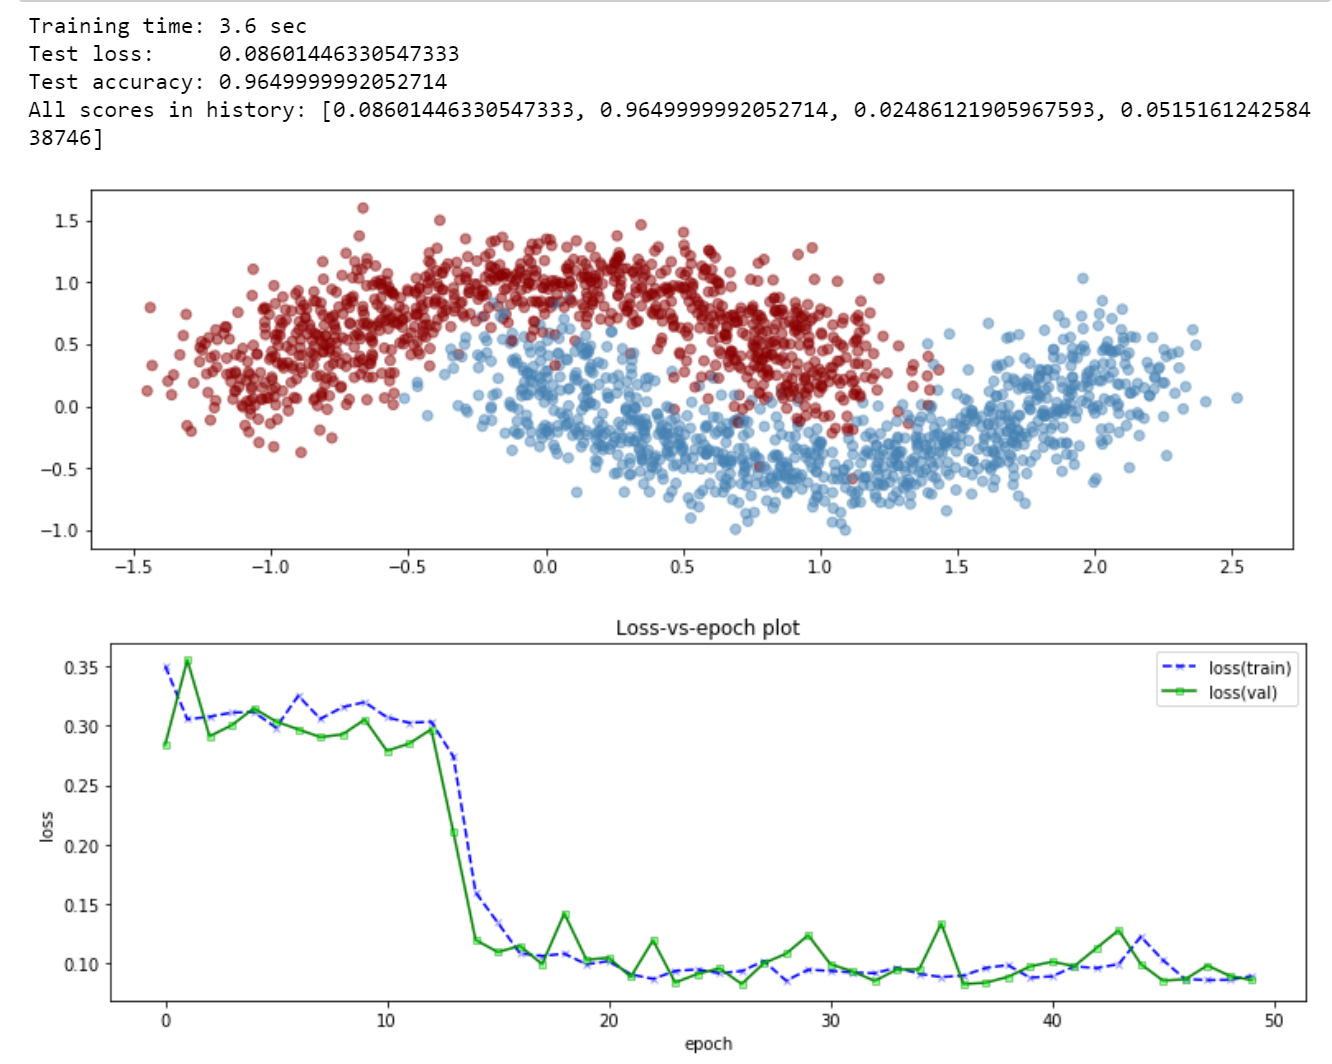
\includegraphics[width=0.8\textwidth]{keras-moon-a}
    \caption{Output from Keras moon Qa, using the Adam optimizer.}
    \label{fig:keras-moon-a}
\end{figure}
\begin{figure}[H]
  \centering
    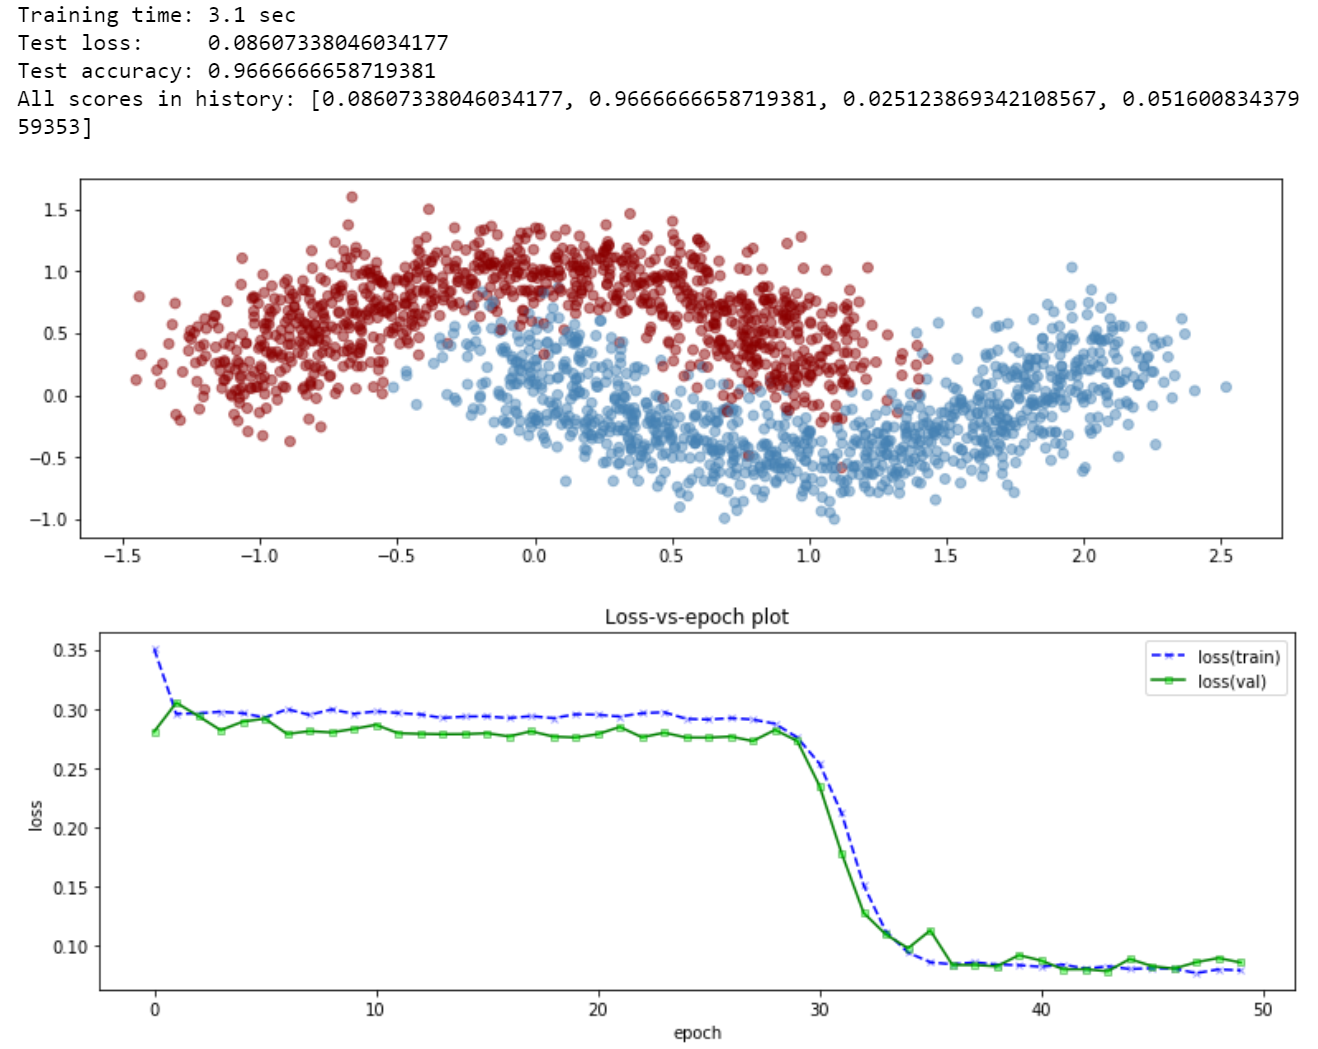
\includegraphics[width=0.8\textwidth]{keras-moon-a-sgd}
    \caption{Output from Keras moon Qa, using the SGD optimizer, using Nesterov Momentum.}
    \label{fig:keras-moon-a-sgd}
\end{figure}

\noindent
Now with the 

\subsection{Qb Keras and Classification Categories}
\paragraph{One-Hot encoding} was first presented to us i chapter 2, page 63. It is a usefull tool when working with categorial values, especially when they do not introduce a natural ordering like: "First", "Second" and "Third" where these could then just be transformed into numerical values: 0, 1 and 2, which is also know as interger encoding. 
\\ \\
But when there is no natural odering like colors: "Red", "Green" and "Blue", we instead use \textbf{One-Hot} encoding, which would then the case of the colors, create a binary table, so \textbf{Red} = 1,0,0 and \textbf{Green} = 0,1,0 and \textbf{Blue} = 0,0,1.
Then with a logic gate aproach the model can distinct each of the categories. That is what the \textbf{to\_categorical} method does, it takes the catogries and one-hot encodes them returning a binary matrix representing the categories, as it is explained in the keras "Utils" documentation.

\newline
\paragraph{categorical\_accuracy} function allows parsing the \textbf{y\_pred} vector with our predictions and a vector with \textbf{y\_true} which represents the "feature" labels to measure the accuracy against. In contrast to the normal accuracy, this only measures whether feature label is correct or not.

\subsection{Qc Optimize the Keras Model}
In this part of the exercise we are supposed to experiment with the different parameters adding layers, increasing epochs, basically adjusting the different hyper-parameters to see if there are any noticeable effects.
\\ \\
This time the Adam optimizer is the only one used and instead of testing different classifiers, focus was on tuning other paramerters. To start with increasing the \textit{EPOCHS} from 50 to 100.
This did not create any real noticeable change, the training time took about twice as long, which i was to be expected. But the accuracy score changed by little less than 1 percent increase.
\\ \\
Then trying to add \textbf{epislon = 0.5} parameter to the model which by the documentations explanation adds a "fuzz-factor". This did make a noticeable change, but for the worse however. It lowered the accuracy by quite a bit. It went down from 96.4 percent to 88.5. And the test loss went up by quite a big amount, from 8.6 percent test loss, to 27.7 percent. Which also explains why the decision boundary basically flat-lines through the data set as seen in figure \ref{fig:keras-moon-c-epsilon}. Further increasing the epsilon value continued to produce worse results.

\begin{figure}[H]
  \centering
    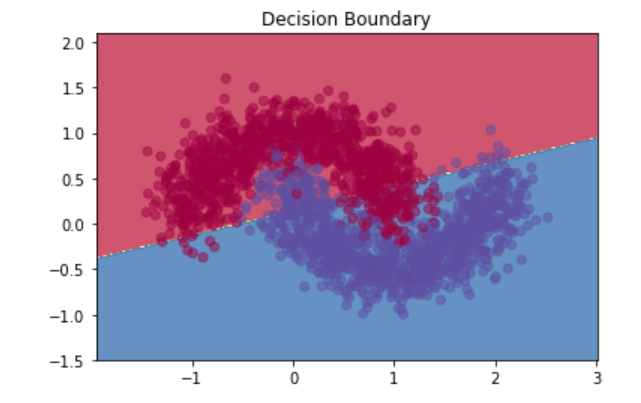
\includegraphics[width=0.8\textwidth]{keras-moon-c-epsilon}
    \caption{Adding epislon fuzz factor to the Adam optimizer.}
    \label{fig:keras-moon-c-epsilon}
\end{figure}
\noindent
Then trying to change the activation layer from \textbf{activation="softmax"} to \textbf{activation="relu"} increased the accuracy by a mere 0.2 percent, but also increased the test loss, it made it fluctuate more. And again trying to add another layer with 2 neurons and sigmoid only made it worse by a tiny margin.

\\ \\ In the end what made the best result and where we chose to stop. Was changing the first activation layer to \textbf{activation="relu"} and then the second layer to \textbf{activation=sigmoid} instead of softmax. These 2 changes increased the accuracy by 0.8 percent and lowered the test-loss by about 1.1 percent.


\end{document}